\begin{figure}
    \tikzset{cross/.style={cross out, draw=red, fill=none, minimum size=2*(#1-\pgflinewidth), inner sep=0pt, outer sep=0pt}, cross/.default={2pt}}
    \centering
    \begin{tikzpicture}[overlay, remember picture]
        \tikzstyle{arc}=[-stealth, very thick, shorten >=2pt, shorten <=2pt];
        \tikzstyle{vertex}=[circle, draw=blue, fill=blue!30];
    
        % HENK EN INGRID
        \onslide<+->{
            \node[label=below:Patient $A$] (henk) at ($(current page.north)+(-3,-2.5)$) {
\includegraphics[width=2cm, height=2cm]{./Figures/Pictures/henk.png}};
            \node[label=below:Donor $A$] (ingrid) at ($(current page.north)+(1,-2.5)$) {
\includegraphics[width=2cm, height=2cm]{./Figures/Pictures/ingrid.png}};
            \node (space) at ($(ingrid.east)+(4,0)$) {.};
            }
    
        \draw<+>[arc] (ingrid.west) -- node[midway] {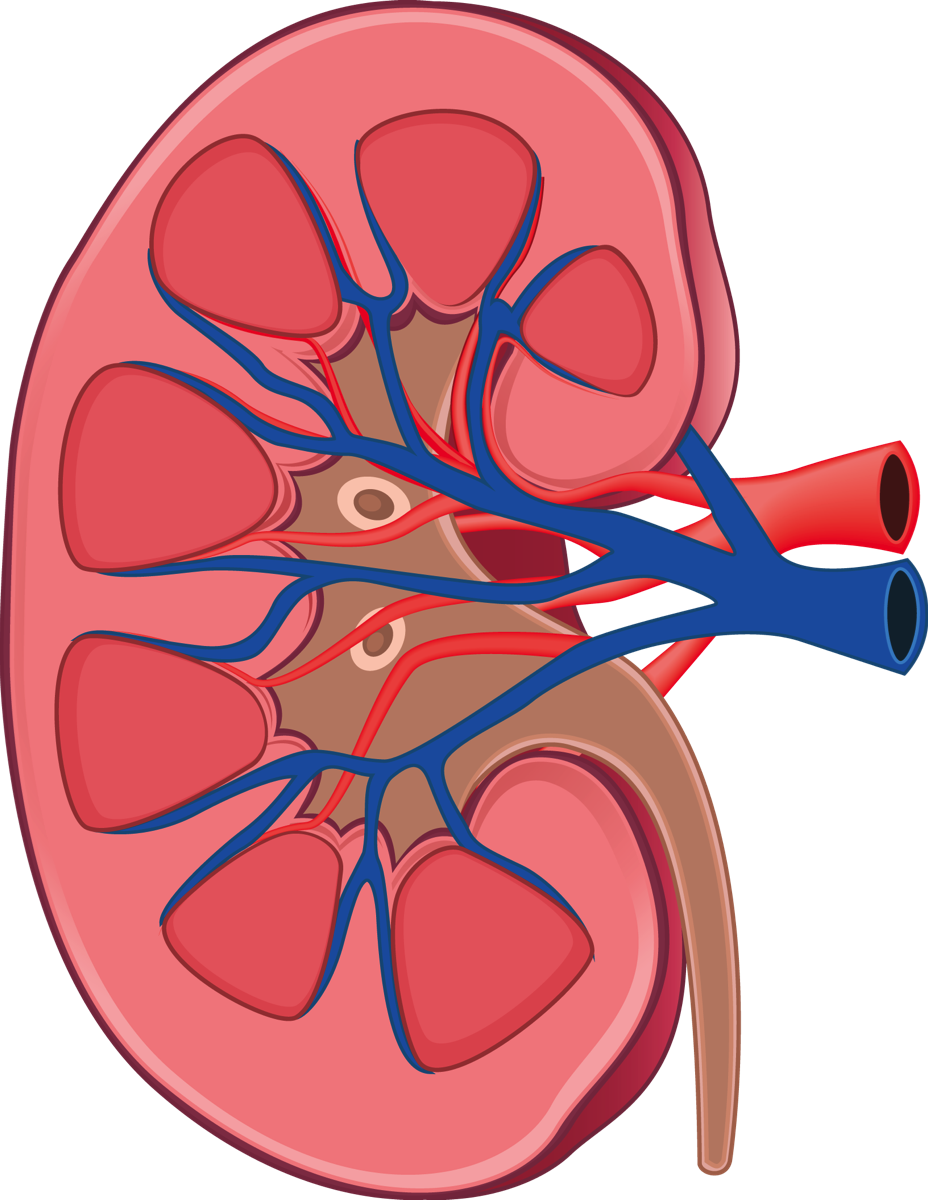
\includegraphics[width=10pt]{./Figures/Pictures/kidney.png}} (henk.east);
        
        \onslide<+->{
            \draw[arc, red] (ingrid.west) -- (henk.east);
            \draw ($(ingrid.west)!.5!(henk.east)$) node[cross=5pt, ultra thick] {};
        }
    
        % AHMED EN FATIMA
        \onslide<+->{
            \node[label=below:Patient $B$] (fatima) at ($(current page.north)+(-3,-5.5)$) {
\includegraphics[width=2cm, height=2cm]{Figures/Pictures/fatima.png}};
            \node[label=below:Donor $B$] (ahmed) at ($(current page.north)+(1,-5.5)$) {
\includegraphics[width=2cm, height=2cm]{Figures/Pictures/ahmed.png}};
        }
    
        \draw<+>[arc] (ahmed.west) -- node[midway] {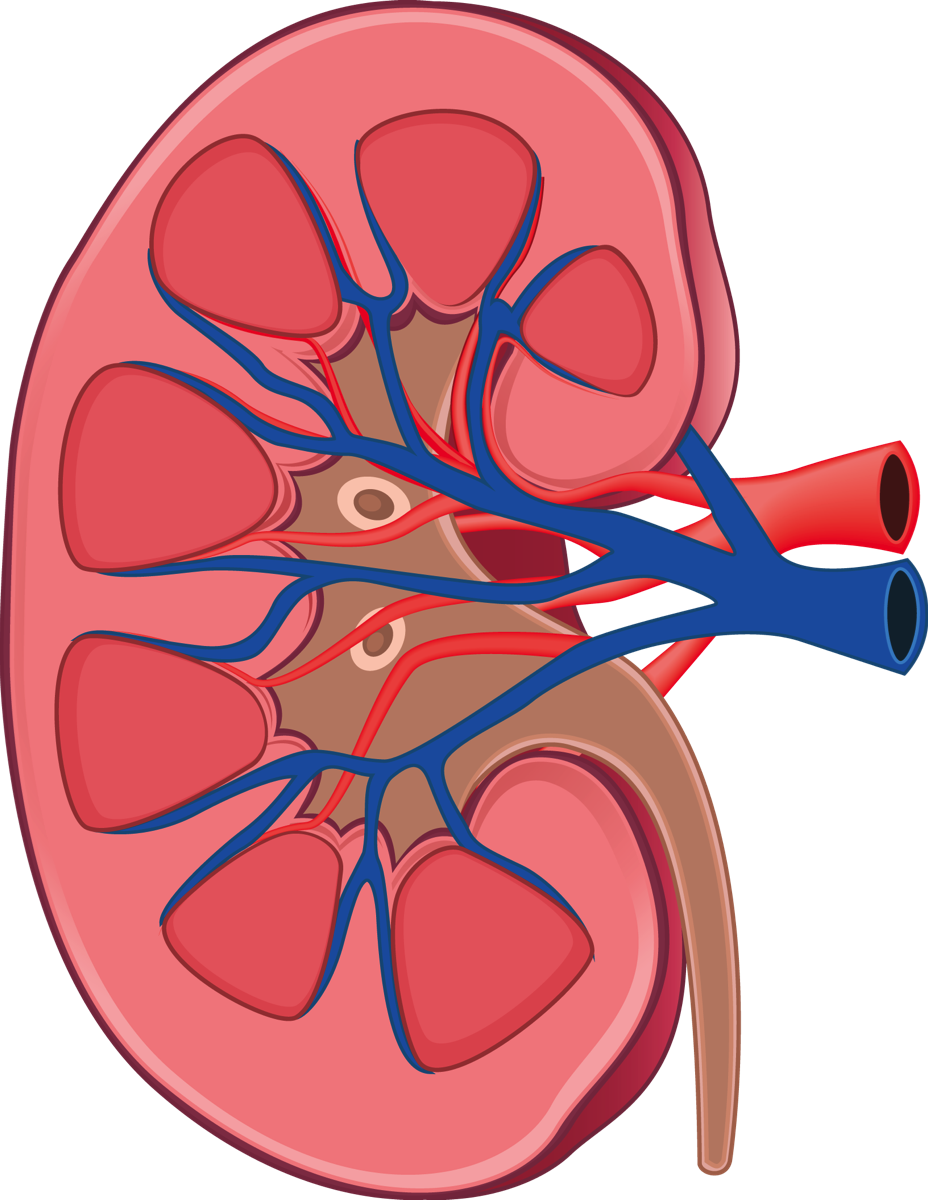
\includegraphics[width=10pt]{./Figures/Pictures/kidney.png}} (fatima.east);
        
        \onslide<+->{
            \draw[arc, red] (ahmed.west) -- (fatima.east);
            \draw ($(ahmed.west)!.5!(fatima.east)$) node[cross=5pt, ultra thick] {};
        }
    
        \onslide<+->{
            \draw[arc, green] (ahmed.160) -- node[pos=0.25, sloped]{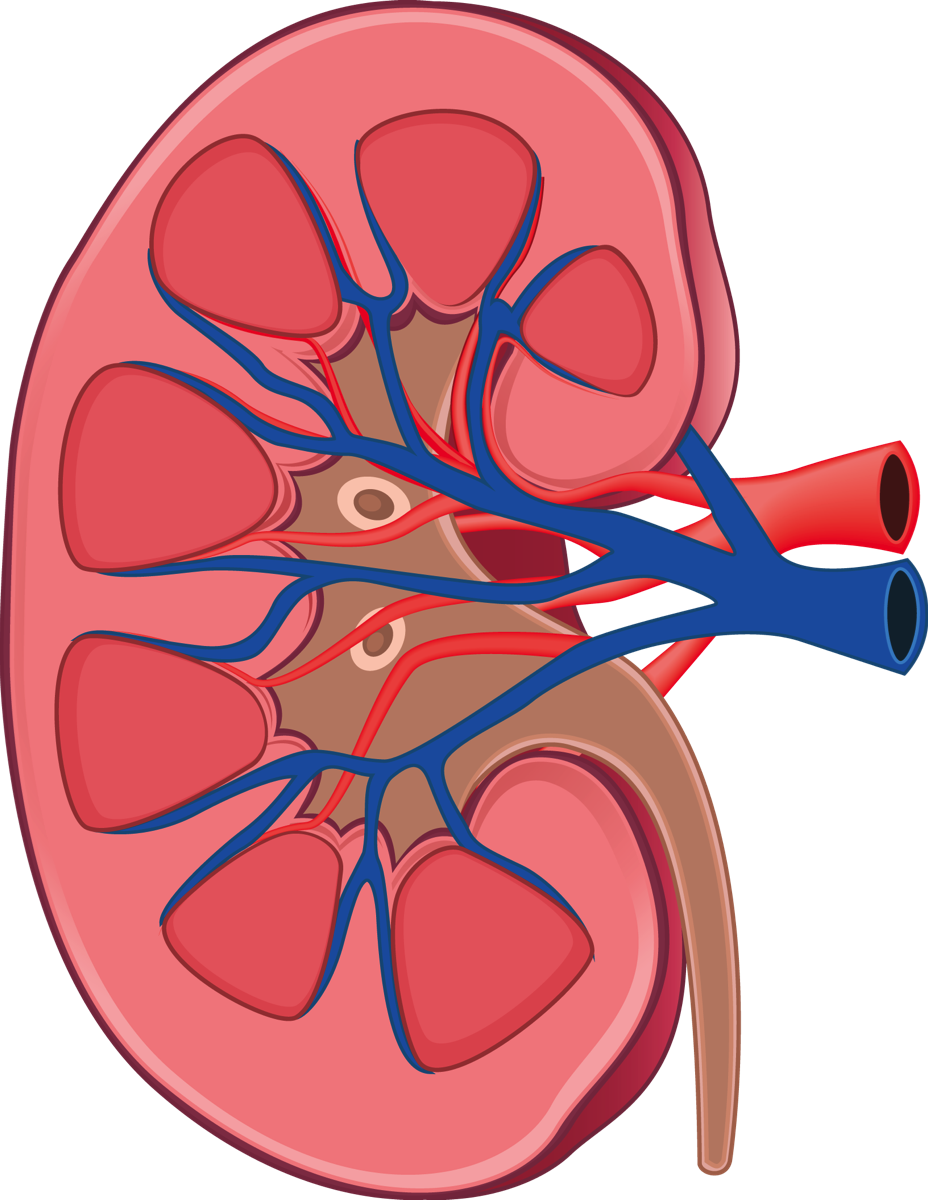
\includegraphics[width=10pt]{./Figures/Pictures/kidney.png}} (henk.320);
            \draw[arc, green] (ingrid.200) -- node[pos=0.25, sloped]{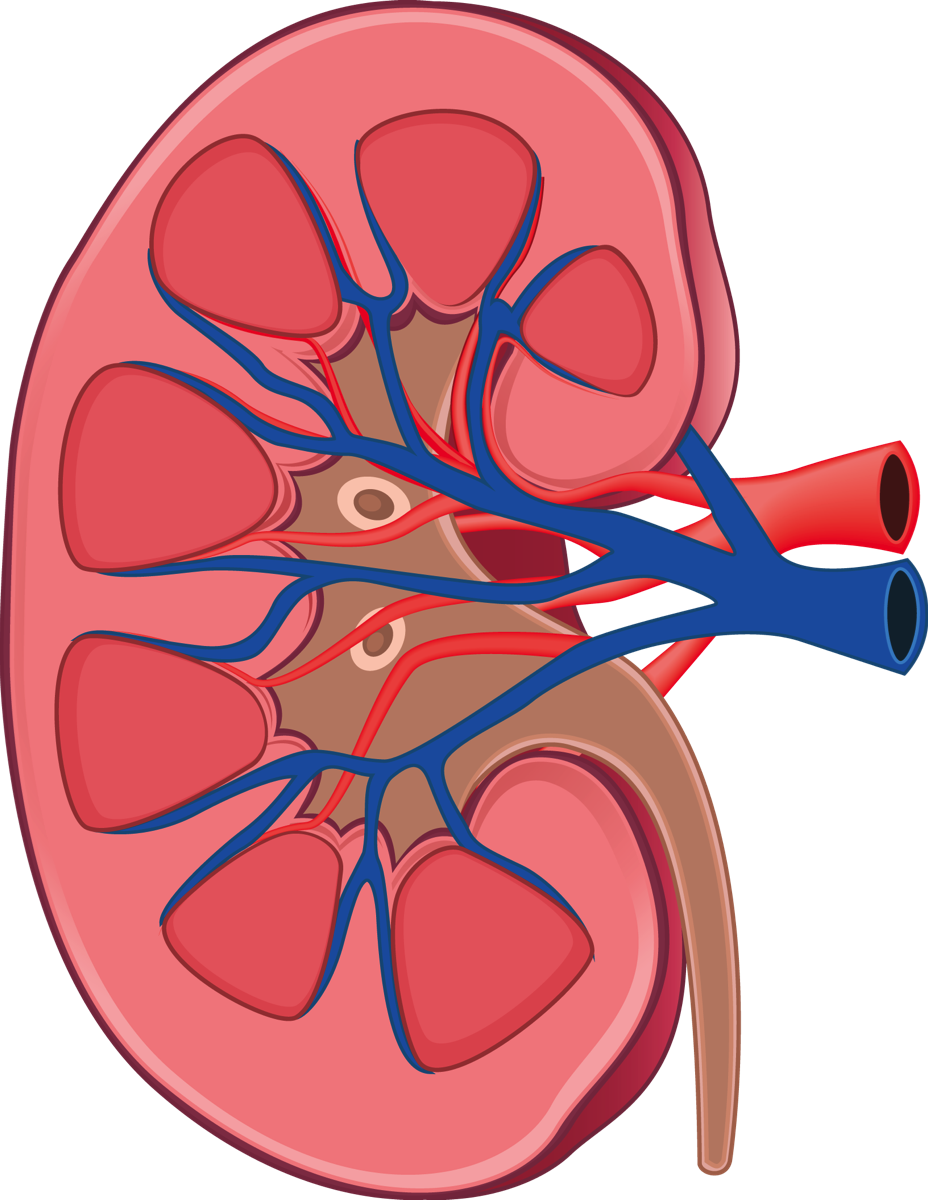
\includegraphics[width=10pt]{./Figures/Pictures/kidney.png}} (fatima.40);
        }
    
        \onslide<+->{
            \node[vertex, label=90:{$p_{A} = (r_{A}, d_{A})$}] (pairhi) at ($(ingrid.east)+(2,0)$) {};
            
            \node[vertex, label=270:{$p_{B} = (r_{B}, d_{B})$}] (pairfa) at ($(ahmed.east)+(2,0)$) {};
    
            \draw[arc, bend right=20] (pairhi.south west) to (pairfa.north west);
            \draw[arc, bend right=20] (pairfa.north east) to (pairhi.south east);
            
        }
    \end{tikzpicture}

\end{figure}
